% Supplement-only insertion; manuscript-relative figure path.
\begin{figure*}[t]
\centering
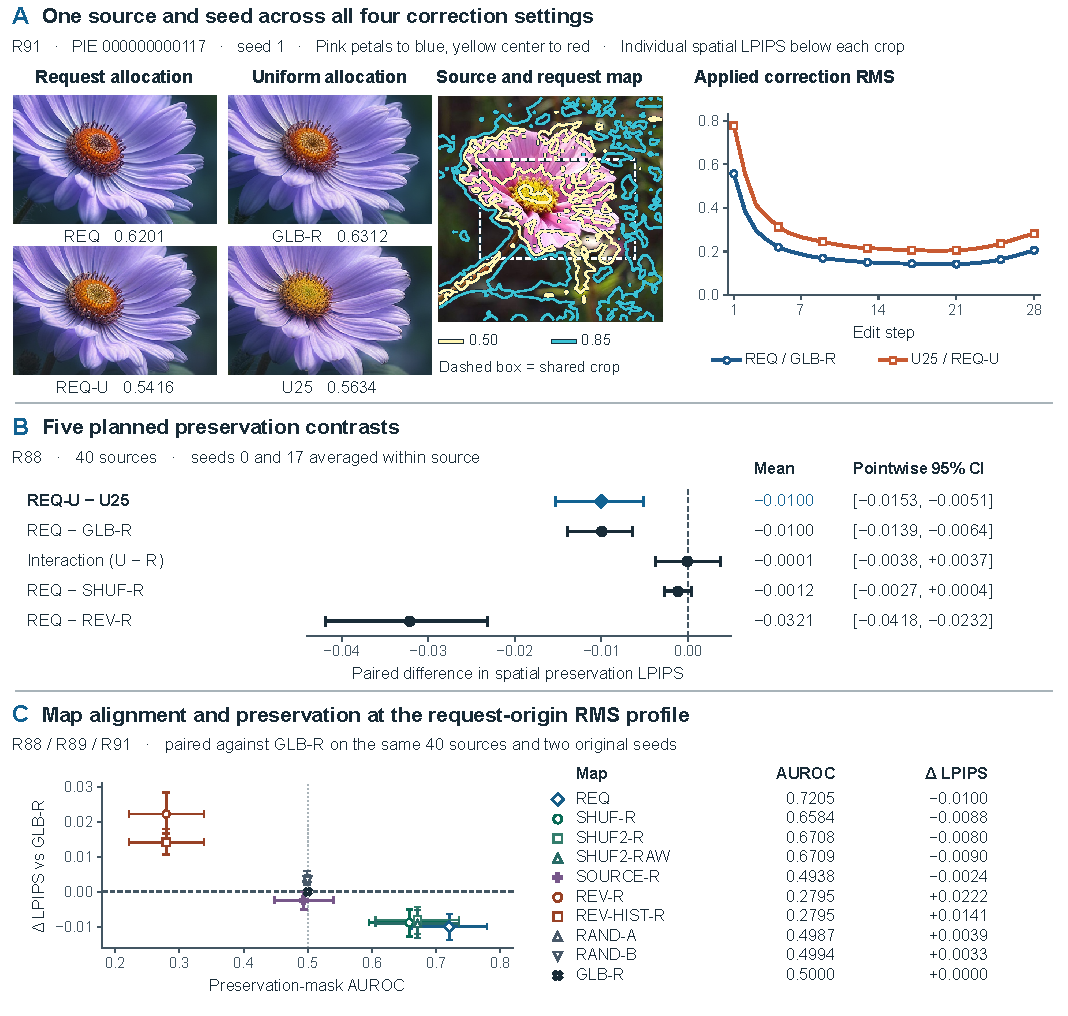
\includegraphics[width=.96\textwidth]{figures/v19_corrector_controls.pdf}
\caption{Source-corrector controls on the common spatial preservation LPIPS scale.
(A) All four native outputs use the same crop of a $512\times512$ image. Each score uses the complete preservation mask. The upper and lower rows use the request- and uniform-origin RMS profiles, respectively. Contours show two levels of the recorded request weight on the source. Lines trace the two native profiles, and open symbols mark every fourth replay step and the endpoint. The largest discrepancy over all 28 steps is $2.98\times10^{-8}$.
(B) The diamond marks the historical primary contrast. The historical interaction subtracts the request-profile allocation contrast from the uniform-profile contrast. Bars are the archived pointwise 95\% category-stratified paired-source bootstrap intervals.
(C) For each applied map, the abscissa gives the AUROC for predicting the official preservation mask. The ordinate gives the paired LPIPS difference from GLB-R, whose constant weights give AUROC 0.5. Negative differences favor the named map. Horizontal and vertical intervals are marginal 95\% category-stratified source bootstraps (20,000 draws). Each source contributes its mean over seeds 0 and 17.}
\label{fig:v19-corrector-controls}
\end{figure*}

The first shuffled donor (SHUF-R) gives a mean AUROC of 0.6584 and a preservation LPIPS difference of $-0.0088$ from GLB-R. The correct request map gives 0.7205 and $-0.0100$, respectively. The two reversed maps have nearly identical mean AUROC (0.2795) and different LPIPS penalties ($+0.0222$ and $+0.0141$). The protection-floor runs use the uniform-origin profile on 20 sources and are reported separately.
